\chapter{
نتایج جدید
}
\section{مقدمه}
در این فصل ابتدا به بررسی مقاله
\cite{arya}
 می‌پردازیم. این مقاله پایه تحقیقاتی نتایج جدید به دست آمده است. مزومدار در این مقاله با تعریف مسئله‌ی 
 \transf{
 سیستم ذخیره‌سازی توزیع شده با قابلیت بازیابی محلی تک-شکست
 }{
 single-failure locally recoverable distributed storage system
 }
اثبات می‌کند این مسئله‌ی دوگان مسئله‌ی کدگذاری اندیس است.

سپس با تعمیم مسئله‌ی سیستم ذخیره سازی و معرفی مسئله‌ی
\transf{
	کدگذاری منبع انعطاف پذیر
}{PSIC: Pliable source index coding}
 نشان اثبات می‌کنیم مسئله‌ی تعمیم یافته دوگان مسئله‌ی کدگذاری اندیس منعطف در حالت خطی  است.
\newpage

\section{
 سیستم ذخیره‌سازی توزیع شده با قابلیت بازیابی محلی تک-شکست
}
در این بخش به مروری کلی از مقاله مزومدار، که پایه علمی نتایج جدید به دست آمده است، می‌پردازیم.

یکی از چالش‌ها در سیستم‌های ذخیره سازی داده توزیع شده، بازیابی داده‌های از دست رفته به دلیل خراب شدن یکی از سرورها است. 
برای حل این مشکل هر داده در چندین سرور ذخیره می‌شود تا در صورت از بین رفتن یکی از سرورها داده‌ها آن سرور از دست نرود. چالش این روش هزینه‌ی بازیابی سرور از دست رفته است. یعنی زمانی که سرور خراب شده را جایگزین می‌کنیم و قصد داریم داده‌ها سرور قبلی را روی سرور جدید قرار دهیم باید آن داده‌ها را از بقیه سرورهای شبکه 
\transf{
دریافت
}{download}
کنیم. اما هزینه‌ی دریافت یک داده از سرورهای مختلف متفاوت است.
``در سیستم‌های توزیع شده خراب شدن یک تک سرور متداول ترین مشکل است.``

``مطالعه‌ی سیستم‌های ذخیره سازی با قابلیت بازیابی اولین بار در
\cite{5550492}
مورد توجه قرار گرفت. در چندین کار جدید این مسیر ادامه پیدا کرد. در
\cite{6259860}
توصیف مرتبی برای
\transf{
ویژگی بازیابی محلی
}{locally repairable property}
ارائه می‌شود. نتایج این مقاله در جهت‌های مختلف توسعه داده شده است و حتی نتایجی از جنس غیرممکن بودن نیز کشف شده است(برای مثال به
\cite{
	6570829, kamath2013codes,6818438,silberstein2013optimal, tamo2013optimal}
و به خصوص مقاله اخیر 
\cite{Tamo_2014}
رجوع کنید.). نکه قابل توجه در مقالات بالا عدم توجه به توپولوژی شبکه است و به تمام سرور ها بدون در نظر گرفتن محل فیزیکی آن‌ها نزدیک به هم دیگر و ارتباطاتشان با بقیه سرورها نگاه می‌شود.
 ``
 
 مزومدار در ادامه برای از یک گراف برای در نظر گرفتن توپولوژي واقعی شبکه استفاده می‌کند. هر راس متناظر یک سرور است و هر دو سروری که با هم ارتباط دارند با یک یال به یک دیگر متصل شده اند. سپس اثبات میکند این مدل جدید دوگان مسئله کدگذاری اندیس است.
 
 \subsection{تعریف مسئله}
 شبکه‌ی ارتباطی یک سیستم ذخیره سازی توزیع شده را در نظر بگیرید.
 \ref{fig:storage-graph}
 یک مثال برای چنین شبکه‌ای است. ارتباط بین سرورها بر اساس توانایی ارتباطی آن‌ها است(که میتواند به خاطر فاصله‌ی جغرافیایی ارتباطات فیبر نوری و ...). همچنین ممکن است به خاطر مسائل فنی در تفاوت فنی میان سرورها و ارتباطشان(مثال سرعا متفاوت دانلود و آپلود) از گراف جهت دار استفاده کنیم.
 
 هدف ما این است که اگر یکی از سرورها دچار مشکل شود و دیتای آن از بین برود سرور جایگزین شده در همان نقطه بتواند با گرفتن اطلاعات از سرورهایی که به این نقطه وصل هستند دیتای سرور از دست رفته را بازیابی کند.
 
 با داشتن شبکه‌ی سرورها بیشترین مقدار اطلاعاتی که می‌توان در شبکه ذخیره کرد چقدر است؟
\begin{figure}[H]
	\centering
	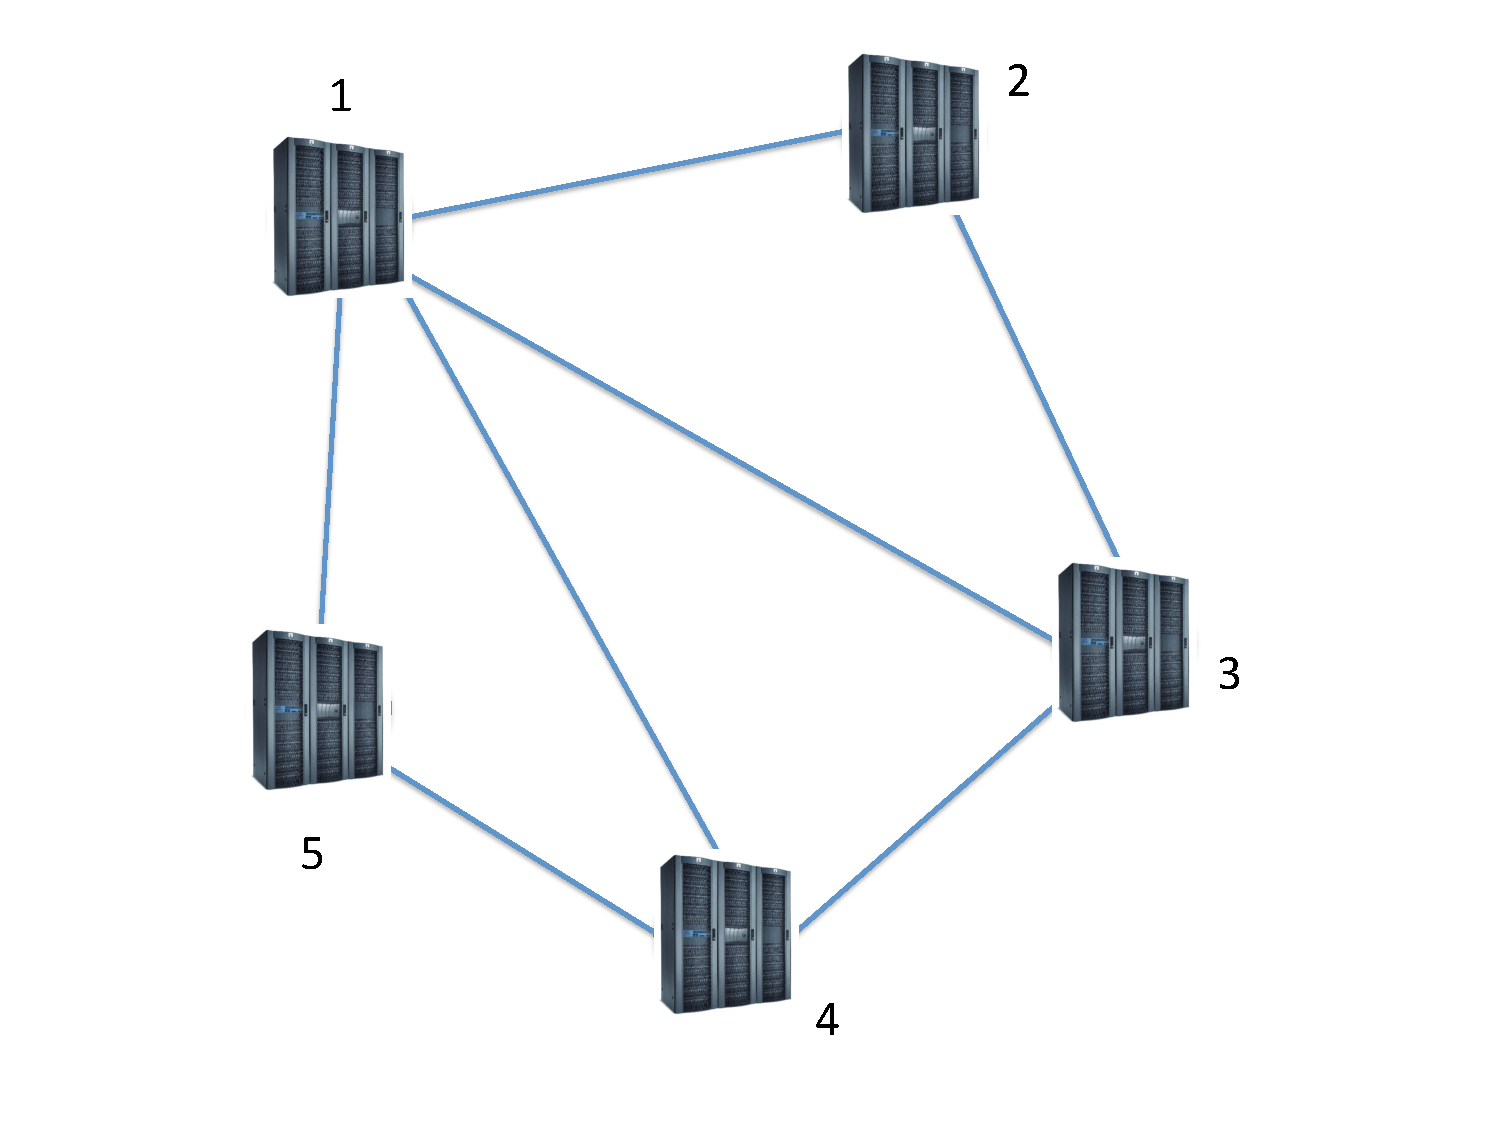
\includegraphics[width=0.5\linewidth]{figs/chapter6/storage-graph}
	\caption{
		مثالی از یک شبکه ارتباطی سرورهای یک سیستم ذخیره‌سازی توزیع شده
		\cite{arya}
		}
	\label{fig:storage-graph}
\end{figure}

\begin{definition}[
	\transf{
	کد ذخیره سازی توزیع شده قابل بازیابی
	}{ًRDSS-code}
	]
	برای گراف جهت‌دار
	$G(V, E)$
	که
	$V = \{1, \ldots, n\}$
	و
	$N(i)$
	همسایه‌های راس
	$i$
	است و میدان
	$\mathbb{F}_{q}$
	و متغیرهای تصادفی
	$X_1, X_2, \ldots, X_m \in \mathbb{F}_{q}$
		کد ذخیره سازی توزیع شده قابل بازیابی 
		$\mathcal{C} \subseteq \mathbb{F}_{q}$
		مجموعه‌ای از بردار‌ها از
		$\mathbb{F}_{q}$
		همراه با مجموعه‌ی توابع قطعی بازیابی به شکل
		$f_i: \mathbb{F}_q^{|N(i)|} \to \mathbb{F}_q$
		به طوری که برای هر مجموعه از متغیرهای تصادفی 
		$(X_1, X_2,\dots,X_n) \in \mathbb{F}_q^n$
		داشته باشیم:
		$$X_i = f_i(\{X_j: j \in N(i)\}), \quad i = 1,\dots,n$$
\end{definition}

به
$\log_q(|C|)$
\transf{
بعد کد
}{dimension of code}
 گفته می‌شود. برای گراف داده شده‌ی $G$ بزرگترین بعد کد را با
 $RDSS_q(G)$
 نشان می‌دهیم.
  \begin{definition}
  	
  	میگوییم ماتریس
  	$A_{n \times n} = (a_{ij}), a_{ij} \in \mathbb{F}_q$
  	بر گراف
  	$G(V, E)$
  	\transf{
  		مطابقت
  	}{fits}
  	روی میدان
  	$\fq$
  	میکند اگر 
  	\begin{latin}
  		\begin{align*}
  			& \forall i : a_{ii} \ne 0 \\
  			& \forall i \ne j:  (i, j) \notin E \Rightarrow a_{ij} = 0
  		\end{align*}
  	\end{latin}
  \end{definition}
 \begin{definition}[
 	\transf{
 	رتبه کمینه
 }{minrank}
 	]
 	رتبه کمینه گراف
 	$G$
 	بر روی میدان
 	$\mathbb{F}_q$
 	به صورت زیر تعریف می‌شود:
 	\begin{equation}
 		\minrank_q(G) = \min\{\rank_{\mathbb{F}_q}(A): A \text{ fits } G\}.
 	\end{equation}
 \end{definition}
 \begin{theorem}
 	در
 	\cite{4031356}
 	نشان داده شده است که:
 	\begin{equation}
 		\indx_q(G) \le \minrank_q(G),
 		\label{eq:bary}
 	\end{equation} 
 \end{theorem}
 \begin{example}[
 	توابع خطی
 	\cite{arya}
 	]

 	برای گراف داده شده در
 	\ref{fig:storage-graph}
 	داریم:
 	\begin{align*}
 		N(1) = \{2,3,4,5\}, \, N(2)  = \{1,3\}, N(3)  = \{1,2,4\}, \\
 		N(4)  = \{1,3,5\},  N(5)  = \{1,4\}.
 	\end{align*}
 	اگر داده‌ی درون سرور
 	$i$
 	را با
 	$X_i$
 	نشان دهیم برای اینکه بتوانیم در صورت از دست رفتن یک سرور اطلاعات آن را به صورت محلی بازیابی کنیم باید توابع زیر را داشته باشیم:
 	$X_1 = f_1(X_2,X_3,X_4,X_5), X_2 = f_2(X_1,X_3), X_3 = f_3(X_1,X_2,X_4), X_4 = f_4(X_1,X_3, X_5), X_5 = f_5(X_1, X_4).$

 	فرض کنید توابع
 	$f_i$
 	همگی خطی هستند پس برای
 	$\alpha_{ij} \in  \mathbb{F}_q, 1\le i,j\le 5,$
 	خواهیم داشت:
 	 	\begin{align*}
 		X_1 &= \alpha_{12} X_2 +\alpha_{13} X_3 + \alpha_{14}X_4 + \alpha_{15}X_5\\
 		X_2 &= \alpha_{21}X_1+\alpha_{23}X_3\\
 		X_3 &= \alpha_{31}X_1 +\alpha_{32}X_2+\alpha_{34}X_4\\
 		X_4 &= \alpha_{41}X_1 + \alpha_{43}X_3 + \alpha_{45}X_5\\
 		X_5 &= \alpha_{51}X_1+\alpha_{54}X_4.
 	\end{align*}
 	که نتیجه خواهد داد که
 	$(X_1,X_2,\dots, X_5)$
 	در فضای پوچ ماتریس
 	\[
 	D \equiv
 	\left( \begin{array}{ccccc}
 		1 & -\alpha_{12} & -\alpha_{13}  & - \alpha_{14} & -\alpha_{15} \\
 		-\alpha_{21} & 1 &  -\alpha_{23} & 0 & 0 \\
 		-\alpha_{31} & -\alpha_{32} & 1 & -\alpha_{34} & 0\\
 		-\alpha_{41} & 0 &-\alpha_{43}  & 1 & -\alpha_{45}\\
 		-\alpha_{51} &0 & 0 & -\alpha_{54} & 1
 	\end{array} \right).\] 
 	قرار دارد.
 	
 	بعد فضای پوچ ماتریس برابر
 	$|null(D)| = n - rank(D)$
 	است. پس اگر خود را به توابع خطی محدود کنیم خواهیم داشت:
 	$$RDSS_q(G) = n - minrank_q(G)$$
 	ولی برای توابع غیر خطی این تساوی برقرار نخواهد بود و خواهیم داشت:
 	\begin{equation}
 		\rdss_q(G) \ge n - \minrank_q(G),
 		\label{eq:minrk}
 	\end{equation}
 	این نامساوی و نامساوی
 	\ref{eq:bary}
 	این حدس را به ما میدهد که
 	$\rdss_q(G) = n - \indx_q(G)$
 	ولی متاسفانه همان طور که در مثال بعدی می‌بینیم این حدس درست نیست.
 \end{example}
 
 \begin{example}[
 	تاثیر توابع غیر خطی
 	\cite{arya}
 	]
 	گراف زیر را در نظر بگیرید:
\begin{figure}[H]
	\centering
	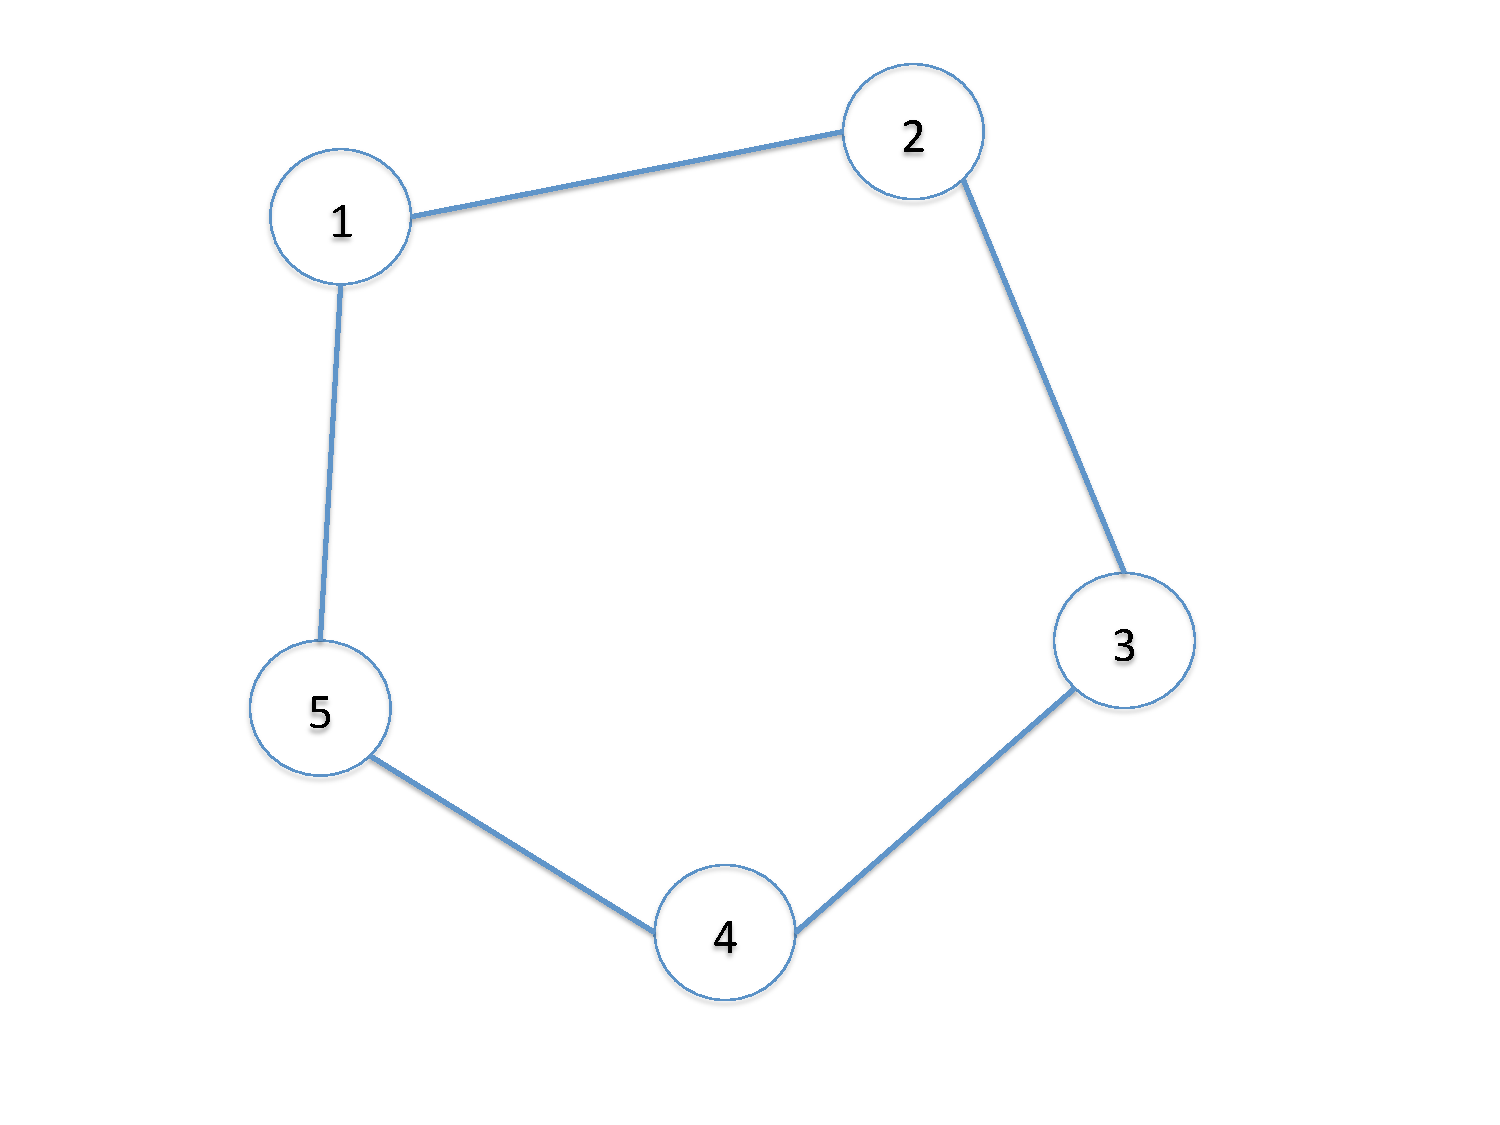
\includegraphics[width=0.7\linewidth]{figs/chapter6/storage-graph-pent}
	\caption{}
	\label{fig:storage-graph-pent}
\end{figure}
بزرگترین کد برای این گراف به شکل زیر است:
$\{00000,01100,00011,11011,11101\}$
که توابع مربوطه به شکل زیر خواهد بود:
\begin{align*}
	X_1 = X_2 \wedge X_5, 
	X_2 = X_1 \vee X_3,
	X_3 = X_2 \wedge \bar{X}_4, \\
	X_4 = \bar{X}_3 \wedge X_5
	X_5 = X_1\vee X_4.
\end{align*}
که نتیجه می‌دهد:
$\rdss_2(G) = \log_2 5$
ولی میدانیم که
$\indx_2(G)=3$.
زیرا اگر فرستند مقادیر
 $Y_1= X_2+X_3, Y_2= X_4+X_5$ 
 و
  $Y_3= X_1+X_2+X_3+X_4+X_5.$
  را ارسال کند گیرنده‌ها میتوانند با توابع
  $X_1 = Y_1 + Y_2+Y_3; X_2 = Y_1+X_3; X_3 = Y_1+X_2; X_4 = Y_2+X_5; X_5 = Y_2+X_4.$
  پیام‌های خود را بازیابی کنند.
 \end{example}
 
 با وجود آنکه در حالت کلی 
 $\rdss_q(G) \ne n - \indx_q(G)$
 ولی این دو مقدار فاصله‌ی زیادی از هم ندارند. بلکه برای الفباهای با اندازه به اندازه‌ی کافی بزرگ میتوان آن‌ها را به اندازه‌ی دلخواه به هم نزدیک کرد. این نکته از قضیه 
 \ref{thm:aryamain}
 نتیجه می‌شود.
 \begin{theorem}\label{thm:aryamain}
 	برای گراف
 	 $G(V,E)$,
 	 داریم
 	\begin{align}
 		n - &\rdss_q(G) \le \indx_q(G) \le n -\rdss_q(G)\nonumber \\
 		&  + \log_q\Big(\min\{n\ln q, 1+ \rdss_q(G)\ln q \}\Big). 
 	\end{align}
 \end{theorem}
 
 این قضیه در
 \cite{4691014}
 با ابزار های نظریه‌ی گراف اثبات می‌شود . مزومدار در ادامه با اثباتی الگوریتمی این قضیه ثابت می‌کند. از آنجایی که اثبات این قضیه کاربردی در نتایج جدید ما ندارد از تکرار آن پرهیز می‌کنیم.

 
\section{نتایج جدید}\label{sec3}
در این بخش، ابتدا به طور رسمی مسئله کدگذاری منبع انعطاف پذیر را تعریف می‌کنیم. سپس، قضیه اصلی این مقاله را در مورد ارتباط بین مسئله کد انعطاف پذیر خطی (PIC) و کد منبع انعطاف پذیر خطی (PSID) بیان می‌کنیم.
\subsection{
		کدگذاری منبع انعطاف پذیر
}
\begin{recal}
	دلیل اینکه از نام کدگذاری اندیس برای مسئله کدگذاری اندیس استفاده شد آن است که می‌توان نگاه متفاوتی به مسئله داشت. در نگاه اول مسئله شامل یک فرستنده و تعدادی گیرنده است که گیرنده‌ها به دنبال داده‌ی جدیدی هستند و وظیفه‌ی فرستنده است که با ارسال پیام‌هایی آن‌ها را آگاه کند. اما نگاه دیگری نیز وجود دارد. در نگاه قبل ما دو عنصر اصیل در مسئله داشتیم. فرستنده و گیرنده‌ها(و البته اطلاعات جانبی گیرنده‌ها) ولی می‌توان خود پیام‌ها را هم به عنوان یک عنصر اصلی در مسئله دید.
	
فرض کنید 
$n$
پیام‌ از
$\mathbb{F}_q$
 داریم. قبل از مشخص شدن پیام‌ها فرستنده و گیرنده‌ها تعدادی مجموعه به شکل
 $\forall i \in [k]: A_i \subseteq \fq$
 مشخص میکنند که اجتماع آن‌ها کل فضای پیام‌ها را پوشش دهد یعنی:
 $ \bigcup\limits_i^k A_i = \fq^n $
 و علاوه بر آن اگر هر گیرنده بداند پیام‌ها در کدام
 $A_i$
 است بتواند بر اساس اطلاعات جانبی خود پیام مورد نظر خود را بازیابی کند. سپس بعد از مشخص شدن پیام‌ها فرستنده تنها اندیس مجموعه‌ی شامل پیام را برای گیرنده‌ها ارسال کند. این کار تنها به
 $\log_q(k)$
 ارسال پیام از طرف فرستنده نیاز دارد.
\end{recal}
\begin{example}
	\cite{ourwork}
	فرض کنید پیام‌ها از
	$\mathbb{F}_2$
	می‌آیند یعنی
	$X_i \in \{0, 1\}$
	برای گراف اطلاعات جانبی زیر چند فرستنده چه پیام‌هایی می‌تواند بفرستد؟
	\newline
		\begin{minipage}{0.5\textwidth}
			
				\begin{figure}[H]
					\centering
				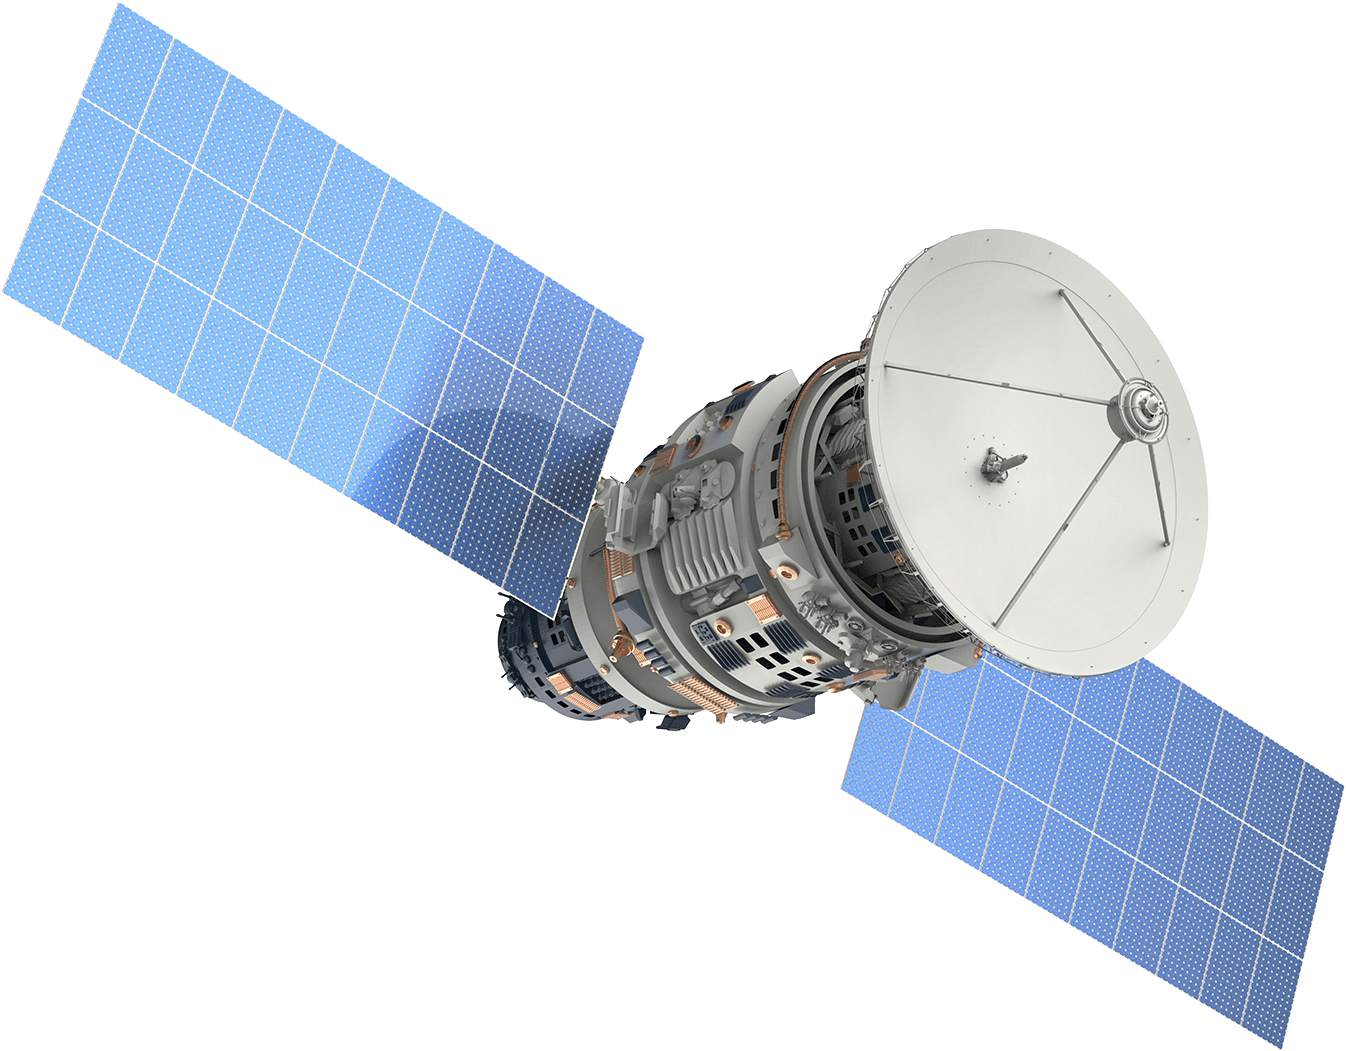
\includegraphics[width=0.3\linewidth]{figs/chapter6/satelite}
			\end{figure}
		\begin{enumerate}
		\item\centering$Y = (X_1,X_2,X_3)$
		\item \centering$Y = (X_1 + X_2 + X_3) $
\end{enumerate}
	\end{minipage}
		\begin{minipage}{0.5\textwidth}
		\centering
		\begin{tikzpicture}[->, >=stealth, auto, semithick]
			% Set the positions of the nodes
			\node[circle, draw=blue, fill=blue!20, inner sep=0pt] (C1) at (0,2) {
					
\includegraphics[width=0.06\linewidth]{figs/chapter6/thinkingemoji.png}
			};
			\node[circle, draw=blue, fill=blue!20, inner sep=0pt] (C2) at (1.5,2) {
					
\includegraphics[width=0.06\linewidth]{figs/chapter6/thinkingemoji.png}
			};
			\node[circle, draw=blue, fill=blue!20, inner sep=0pt] (C3) at (3,2) {
					
\includegraphics[width=0.06\linewidth]{figs/chapter6/thinkingemoji.png}
			};
			\node[above] at (1.5,2.5) {We want to know more};
			
			
				\node[circle, draw=green, fill=green!20, inner sep=0pt] (B1) at (0,0) {$B_1$};
				\node[circle, draw=green, fill=green!20, inner sep=0pt] (B2) at (1.5,0) {$B_2$};
				\node[circle, draw=green, fill=green!20, inner sep=0pt] (B3) at (3,0) {$B_3$};
				\node[below] at (1.5,-0.5) {messages};
			
			
				% Draw the edges
				\draw (C1) -- (B1);
			%	\draw[->, color=red]  (C1) -- (B2);
				\draw (C1) -- (B3);
				
				\draw (C2) -- (B1);
				\draw (C2) -- (B2);
			%	\draw[->, color=red]  (C2) -- (B3);
				
		%		\draw[->, color=red]  (C3) -- (B1);
				\draw (C3) -- (B2);
				\draw (C3) -- (B3);
			
			% Position the parts
			\begin{scope}[on background layer]
				\node[fit=(C1) (C2) (C3), draw=blue, fill=blue!10, rounded corners] {};
				\node[fit=(B1) (B2) (B3), draw=green, fill=green!10, rounded corners] {};
			\end{scope}
		\end{tikzpicture}			
	\end{minipage}
	\newline
		فرستنده می‌تواند در روش اول با سه ارسال نیاز تمام گیرنده‌ها را ارضا کند. در روش دوم تنها با یک ارسال این کار را انجام می‌دهد. زیرا هر گیرنده با استفاده از توابع زیر می‌تواند پیام مورد نظر خود را بازیابی کند:
	\begin{align*}
		\begin{cases}
				X_1 &= Y - X_2 - X_3 \\
				X_2 &= Y - X_1 - X_3  \\
				X_3 &= Y - X_1 - X_2  
			\end{cases}   
	\end{align*}
	با توجه به بحث بالا در مورد نحوه‌ی نگاه به مسئله می‌توان دید که در واقع فرستنده پیام‌ها را به دو دسته تقسیم می‌کند.
	\begin{latin}

		\begin{enumerate}
			\centering
			\item $\{X: X_1 + X_2 + X_3 = 1\}$
			\item $\{X: X_1 + X_2 + X_3 = 0\}$
		\end{enumerate}
	\end{latin}
	حال هر کدام از گیرنده‌ها بر اساس اینکه پیام در کدام دسته است می‌توانند پیام مورد نظر خود را بازیابی کنند.
\end{example}

همان طور که در مثال قبل دیدیم مسئله کدگذاری اندیس را می‌توان به نوعی مسئله‌ی دسته بندی فضای پیام‌ها دید. بر اساس همین ایده مسئله کدگذاری منبع را تعریف میکنیم. در مسئله کدگذاری منبع انعطاف‌پذیر، هیچ فرستنده‌ای وجود ندارد که به گیرنده‌ها بگوید کدام قسمت $X$ انتخاب شده است. به جای آن، مجموعه‌ای از بردارهای $\mathbb{F}^m$ وجود دارد که به این مجموعه
\transf{
کتاب کد
}{code book}
 (یا 
 \transf{
 جدول
 }{table}
 ) گفته می‌شود که $X$ به آن تعلق دارد. سپس، با توجه به اطلاعات جانبی و کتاب کد، هر گیرنده باید پیام مورد نظر خود را بازیابی کند.
\begin{مشاهده}
	مسئله‌ی کدگذاری منبع همان مسئله‌ی کد ذخیره سازی توزیع شده قابل بازیابی است! در واقع مسئله‌ی کد ذخیره سازی را نمی توان برای حالت منعطف به صورتی تعمیم داد که هنوز معنا دار باشد.
	
	در واقع نتیجه جدید به دست آمده در این پایان نامه تعمیم نتیجه مزومدار برای حالت منعطف(و همچنین خطی) است.
\end{مشاهده}

\begin{مشاهده}
توجه داشته باشید که در مسئله PIC، هدف کاهش اندازه پیام‌های منتقل شده است در حالی که در مسئله PSIC، هدف افزایش اندازه کتاب کد (جدول قابل استفاده) است. اکنون به طور رسمی یک جدول قابل استفاده را تعریف می‌کنیم.
\end{مشاهده}

\begin{definition}[جدول قابل استفاده]\label{def1}
برای یک الفبای داده شده $\mathbb{F}$ و نمودار اطلاعات جانبی $G$، یک جدول قابل استفاده $T$ مجموعه‌ای است با عناصری از $\mathbb{F}^m$ به طوری که برای هر گیرنده $c_i$ اگر اطلاعات جانبی آن یکسان است در بعضی از عناصر مختلف، حداقل یک شاخص $i$ وجود دارد که در اطلاعات جانبی او نیست و مقدار یکسانی در تمام آن عناصر دارد. یعنی:
\begin{align*}
    \forall i: \exists j \notin S_i: \forall X, X^\prime: X[S_i] = {X^\prime}[S_i]  \Rightarrow X[j] = {X^\prime}[j]
\end{align*}
ما از اصطلاح جدول استفاده می‌کنیم زیرا عناصر این مجموعه را در یک جدول نمایش می‌دهیم. به این ترتیب، هر ستون یکی از متغیرهای $X_i$ را نشان می‌دهد و هر سطر یک پیام ممکن است.
\end{definition}

مسئله کدگذاری منبع انعطاف‌پذیر، PSIC، برای یافتن بزرگترین جدول قابل استفاده ممکن برای یک $G$ داده شده است.

\begin{remark}
    ما همیشه می‌توانیم $\mathbb{F}^n$ را به جدول‌های قابل استفاده تقسیم کنیم، به عنوان مثال هر $X \in \mathbb{F}^n$ را به عنوان یک جدول قابل استفاده با یک ردیف در نظر بگیریم.
\end{remark}

\begin{lemma}
    اگر $G$ یک گراف باشد و $\mathbb{F}^m$ به جدول‌های قابل استفاده مجزا تقسیم شود، آنگاه تابع رمزگذاری که بردار $X \in \mathbb{F}^m$ را گرفته و آن را به شاخص جدول قابل استفاده‌ای که $X$ به آن تعلق دارد رمزگذاری می‌کند، یک راه‌حل معتبر برای مسئله PIC برای گراف $G$ است.
\end{lemma}
\begin{proof}
    گیرنده $c_i$ را در نظر بگیرید. گیرنده $c_i$ $X[S_i]$ را می‌داند. بر اساس تعریف جدول قابل استفاده، شاخص $j$ خارج از $S_i$ وجود دارد که $c_i$ می‌تواند از جدولی که شاخص آن منتقل شده، یاد بگیرد.
\end{proof}

\begin{corollary}\label{cor1}
اگر همه دسته‌بندی‌های پیام ممکن (یعنی $\mathbb{F}^t$) را در $l$ جدول قابل استفاده مختلف تقسیم کنیم، آنگاه می‌توانیم فقط $\lceil \log(l) \rceil$ بیت داده را به کاربران بفرستیم تا شاخص جدول انتخاب شده را پیدا کرده و پیام مورد نظر خود را بیابند.
\end{corollary}

\begin{note}
    در مورد PIC خطی، تابع رمزگذاری $En$ را می‌توان با یک ماتریس توصیف کرد. $\overrightarrow{f}$ توابع خطی هستند. همچنین، اگر سرور $k$ پیام $Y_i = a_{i,1} X_1 + a_{i,2} X_2 \ldots + a_{i,n} X_n$ را ارسال کند، آنگاه
    \begin{equation*}
        En =
        \begin{pmatrix}
            a_{1,1} & a_{1,2} & \cdots & a_{1,n} \\
            a_{2,1} & a_{2,2} & \cdots & a_{2,n} \\
            \vdots  & \vdots  & \ddots & \vdots  \\
            a_{k,1} & a_{k,2} & \cdots & a_{k,n}
        \end{pmatrix}
    \end{equation*}
\end{note}

\begin{definition}[\textbf{جدول قابل استفاده خطی}]
    فرض کنید $\mathbb{F}$ یک میدان متناهی است. یک جدول قابل استفاده $T$ بر روی $\mathbb{F}$ "خطی" نامیده می‌شود اگر ردیف‌های $T$ یک فضای برداری بر روی $\mathbb{F}$ تشکیل دهند.
\end{definition}

مسئله کدگذاری منبع خطی انعطاف‌پذیر، LPSIC، برای یافتن بزرگ‌ترین جدول قابل استفاده خطی ممکن برای یک گراف داده شده $G$ است.

\begin{remark}
    همیشه حداقل یک جدول ممکن خطی وجود دارد، $\{\overrightarrow{0}\}$. در حالت خطی، ما می‌توانیم $\mathbb{F}^n$ را با یک جدول ممکن خطی و هم‌مجموعه‌های آن تقسیم‌بندی کنیم، به سادگی با در نظر گرفتن جدول ممکن خطی و تمامی انتقالات آن. این کار به ما امکان می‌دهد تا تمام $\mathbb{F}^n$ را پوشش دهیم.
\end{remark}

\begin{example}
    $G_1$
    و
    $G_2$
    شکل زیر را در نظر بگیرید.
    برای
    $G_1$
    می‌توانیم دسته‌پیام‌ها را در 4 مجموعه مختلف (جدول‌ها) تقسیم‌بندی کنیم. در این مثال، همه آن‌ها جدول‌های ممکن هستند. برای
    $G_2$
    ما یک جدول ممکن خطی داریم و تنها هم‌مجموعه‌ای که با هم
    $\mathbb{F}_2^3$
    را پوشش می‌دهند:
    
	\begin{minipage}{0.49\textwidth}
	\centering
    \definecolor{myblue}{RGB}{80,80,160}
    \definecolor{mygreen}{RGB}{80,160,80}
    \begin{tikzpicture}[->, >=stealth, auto, semithick]
        % Set the positions of the nodes
        \node[circle, draw=blue, fill=blue!20, inner sep=0pt] (C1) at (0,2) {$C_1$};

        \node[circle, draw=blue, fill=blue!20, inner sep=0pt] (C2) at (1.5,2) {					$C_2$				};
        \node[circle, draw=blue, fill=blue!20, inner sep=0pt] (C3) at (3,2) {$C_3$				};

        \node[circle, draw=green, fill=green!20, inner sep=0pt] (B1) at (0,0) {$B_1$};
        \node[circle, draw=green, fill=green!20, inner sep=0pt] (B2) at (1.5,0) {$B_2$};
        \node[circle, draw=green, fill=green!20, inner sep=0pt] (B3) at (3,0) {$B_3$};


        % Draw the edges
        \draw (C1) -- (B2);
        \draw (C1) -- (B3);

        \draw (C2) -- (B1);
        \draw (C2) -- (B3);



        \draw (C3) -- (B1);
        \draw (C3) -- (B2);

        % Position the parts
        \begin{scope}[on background layer]
            \node[fit=(C1) (C2) (C3), draw=blue, fill=blue!10, rounded corners] {};
            \node[fit=(B1) (B2) (B3), draw=green, fill=green!10, rounded corners] {};
        \end{scope}
    \end{tikzpicture}
       \captionof{figure}{}
       	       \end{minipage}
       \begin{minipage}{0.25\textwidth}
			        		\begin{tabular}{|c|}
			        			\hline
			        			000 \\
			        			\hline
			        			001 \\
			        			\hline
			        		\end{tabular}
			        		\captionof{table}{$T_1$}
			        	\end{minipage}
			             \begin{minipage}{0.25\textwidth}
	 		       		\begin{tabular}{|c|}
	 		       			\hline
	 		       			000  \\
	 		       			011   \\
	 		       			110  \\
	 		       			101   \\
	 		       			\hline
	 		       		\end{tabular}
	 		       	\captionof{table}{$T_2$}
	 		       	       				        	\end{minipage}

\end{example}

\begin{lemma}
    فرض کنید $G$ یک گراف دوبخشی روی اجزاء $C, B$ باشد. اگر $(En, I, \overrightarrow{f})$ یک کد نمایه‌ای قابل انعطاف خطی برای $G$ باشد، آنگاه یک LPSIC $(W, J, \overrightarrow{g})$ وجود دارد به طوری که $W  = ker(En)$
\end{lemma}

\begin{proof}
    ابتدا، ایده اثبات را مرور می‌کنیم. برای هر مسئله کدگذاری قابل انعطاف خطی، ترکیب‌های خطی که سرور به کاربران پخش می‌کند را در نظر بگیرید. ضرایب جدول ممکن خطی را تشکیل می‌دهند.

    LPSIC 
    $(W, J, \overrightarrow{g})$
     به شکل زیر تعریف می‌شود: 
     $W = ker(En), \overrightarrow{g}_i = \overrightarrow{f}_i(\overrightarrow{0}, X[S_i]), J = I$
    $span(W)$
     را در نظر بگیرید. اگر تاپل پیام 
     $V$
      از این فضای برداری باشد، آنگاه پیام ارسالی همه صفر خواهد بود چون 
      $En \times V = \overrightarrow{0}$
      . دانستن اینکه 
      $V$ از $span(W)$
       است به این معنی است که کدگذاری ارسالی 
      $\overrightarrow{0}$
       است و از آنجایی که کاربر 
       $i$-ام
        می‌تواند 
       $X[I_i]$
        را در PIC حدس بزند، می‌تواند
         $\overrightarrow{f}_i$ 
        را با 
        $\overrightarrow{0}$ 
        به عنوان کد ارسالی به عنوان تابع رمزگشایی خود استفاده کند. پس 
        $span(W)$
         یک جدول ممکن خطی تشکیل می‌دهد و بنابراین 
        $span(W)$
         یک جدول ممکن خطی است و 
        $(W, J, \overrightarrow{g})$ 
        یک راه‌حل
         LPSIC 
        است.
\end{proof}

\begin{lemma}
    اگر
     $(W, J, \overrightarrow{g})$
      یک LPSIC برای $G$ باشد، آنگاه یک
       LPIC $(En, I, \overrightarrow{f})$
        وجود دارد به طوری که
         $span(En) = W^{\bot}$
\end{lemma}

\begin{proof}
    فرض کنید 
    $r = dim(W)$
     و $\{V_1, V_2, \ldots, V_{n - r} \}$ 
     یک پایه برای فضای $n - r$ بعدی $W^\bot$ باشد. ماتریس کدگذاری $En$ را به عنوان یک ماتریس 
     $(n - r) \times n $
      تعریف کنید که سطرهای آن 
      $V_1, V_2, \ldots, V_{n - r}$
       هستند. واضح است که 
      $span(En) = W^\bot$.
       همچنین، $J = I$ قرار دهید و 
       $\overrightarrow{f}_i(\overrightarrow{R}, En(X[S_i]) = f(En(X[S_i] - R[S_i])) + R[I_i]$ که $\exists! V \in W: V + R = X $.
    اکنون باید اثبات کنیم که کاربر $i$-ام می‌تواند $X[I_i]$ را در هر تاپل پیام بازیابی کند. به بیان دیگر، تاپل‌های پیام متفاوتی با 
    $X[I_i]$‌
    های متفاوت وجود ندارد که با اطلاعات جانبی یکسان برای کاربر
     $i$-ام
      و کد ارسالی یکسان (یعنی
       $En(X)$
       ) باشد. فرض کنید برعکس است. آنگاه 
     $X_1, X_2, i$ وجود دارد به طوری که 
     $En(X_1) = En(X_2)$ و 
     $X_1[S_i] = X_2[S_i]$ اما 
     $X_1[I_i] \neq X_2[I_i]$. فرض کنید 
     $W_1, \ldots, W_t$ زیرمجموعه‌های 
     $W$ باشند. آنگاه بردارهای یکتایی وجود دارد که 
     $X_1 = V_1 + {V^\prime}_1, X_1 = V_2 + {V^\prime}_2$
     ، که در آن 
     $V_1, V_2 \in W$
      و 
      $V^\prime_1 \in W_p, V^\prime_2 \in W_q$.
    بر اساس تعریف جدول ممکن، داریم
     $En(V_1) = En(V_2) = 0$.
    باید اثبات کنیم که کاربر $i$ همیشه می‌تواند پیام $I_i$ را تشخیص دهد. 
    $En(X_1) = En(X_2)$
     به این معنی است که هر دو 
    $X_1, X_2$
     از یک زیرمجموعه هستند، یعنی 
    $V^\prime_1 = V^\prime_2$
    . ما ادعا می‌کنیم که برای هر دو زیرمجموعه متفاوت $W_1, W_2$ داریم: 
    $\forall U_1, U_2: U_1 \in W_1, U_2 \in W_2: En(U_1) \neq En(U_2)$
    . این بدان معنی است که کاربران می‌توانند زیرمجموعه تاپل پیام را از همه زیرمجموعه‌های دیگر تمیز دهند. فرض کنید $W_j$ زیرمجموعه‌ای باشد که 
    $X_1, X_2$
     در آن قرار دارند، آنگاه: 
     $R = U - U^\prime: U, U^\prime \in W_j$. 
     حال، 
     $X_1 - R, X_2 - R$ 
     هر دو در $W$ قرار دارند به این معنی که کاربر می‌تواند بین آنها تمایز قائل شود. اما این یک تناقض است زیرا پس از اضافه کردن $R[I_i]$ به پیام $X[I_i]$، کاربر $i$-ام می‌تواند بین $X_1, X_2$ تمایز قائل شود.
    فقط باقی مانده است تا ادعا را ثابت کنیم. در غیر این صورت فرض کنید. از آنجایی که $En$ خطی است، داریم: 
    $En(U_1) = En(U_2) \Rightarrow En(U_1 - U_2) = 0 \Rightarrow U_1 - U_2 \in W \Rightarrow \exists i: U_1، U_2 \in W_i$
    . اما ما فرض کردیم
     $W_1 \neq W_2$.
\end{proof}

\begin{theorem}
    \label{thm1}
    برای هر گراف اطلاعات جانبی 
    $G$، LPSIC $(W, J, \overrightarrow{g})$
     دوگان جبری خطی
      LPIC $(En, I, \overrightarrow{f})$ 
      است به این معنا که:
    \begin{align*}
    (W, J, \overrightarrow{g}) &= \begin{cases}
                                      W = ker(En)\\
                                      I = J \\
                                      \overrightarrow{g}_i(En(X[S_i])) = \overrightarrow{f}_i(\overrightarrow{0}, En(X[S_i])\\
    \end{cases} \\
    (En, I, \overrightarrow{f}) &= \begin{cases}
                                       span(En) = W^{\bot} \\
                                       J = I \\
                                       \overrightarrow{f}_i(\overrightarrow{R}, En(X[S_i]) = g(En(X[S_i] - R[S_i])) + R[I_i]: \exists! V \in W: V + R = X \\
    \end{cases}
    \end{align*}
    و 
    $dim(W) = n - dim(En)$
     یعنی اگر
     $En: \mathbb{F}^n \rightarrow \mathbb{F}^k$
      و کد-کتاب
      $W$ دارای $l$ توپل پیام باشد پس $\log(l) + k = n$
\end{theorem}
\begin{proof}
    این یک پیامد مستقیم از دو لم آخر است. ما فقط باید برابری ابعاد را نشان دهیم. این از این واقعیت ناشی می‌شود که: $dim(W) + dim(W^{\bot}) = n$.
\end{proof}
